\chapter{Anhang}
\label{cha:anhang}

\begin{lstlisting}[language=XML,caption={XML Code für simplen Prozess},captionpos=b,label={lst:anhang_code_xml}]
<xml xmlns="https://developers.google.com/blockly/xml">
    <block type="PLC_Distribute_ExtendSlide__ON" id="w[,^tOV?1A2pYgamWghr" x="15" y="88">
        <next>
            <block type="instruction_wait" id="FFAUMYks/WAmp_I=ASlj">
                <field name="wait_amount">0.2</field>
                <next>
                    <block type="PLC_Distribute_ExtendSlide__OFF" id=".[Hx1gsNm1`I_?Epql~O">
                        <next>
                            <block type="PLC_Distribute_ConveyerForward__ON" id="6k8D(GT3vcFL96uzt3-+">
                                <next>
                                    <block type="instruction_wait" id="qi(*IulXH*3u9LH3,j`z">
                                        <field name="wait_amount">4.3</field>
                                        <next>
                                            <block type="PLC_Distribute_ConveyerForwa rd__OFF" id="1jdIM*0Nm(ulS29B3{LF"/>
                                        </next>
                                    </block>
                                </next>
                            </block>
                        </next>
                    </block>
                </next>
            </block>
        </next>
    </block>
</xml>
\end{lstlisting}

\begin{lstlisting}[language=JavaScript,caption={Code zur Erstellung des Prozess-Randdaten-Objektes},captionpos=b,label={lst:anhang_code_analyse}]
const allUsedActuatorsRaw = [...$(xml).find('block')]
		.map((el) => dic(el.getAttribute("type")))
		.filter((el) => el !== "instruction_wait");
const usedActuators = [...new Set([...$(xml).find('block')]
		.map((el) => dic(el.getAttribute("type").substring(0, el.getAttribute("type").indexOf("__"))))
		.filter((el) => el !== ""))];

const mbomAnalysis = {
    executionTime: Math.round([...$(xml).find('field[name="wait_amount"]')]
    		.map((el) => Number(el.textContent))
    		.reduce((sum, step) => sum + step)*100)/100,
	usedActuators: usedActuators,
	usedResources: [
		{
			name: "cup",
			amount: allUsedActuatorsRaw.filter((el) => el === "PLC_Distribute_ExtendSlide__ON").length
		},
		{
			name: "lid",
			amount: allUsedActuatorsRaw.filter((el) => el === "PLC_Distribute_Vacuum__ON").length
		}
	],
	nbrOfGroups: $(xml).children('block').length,
	nbrOfBlocks: $(xml).find('block').length
};
\end{lstlisting}
%
\begin{figure}[htbp]
	\centering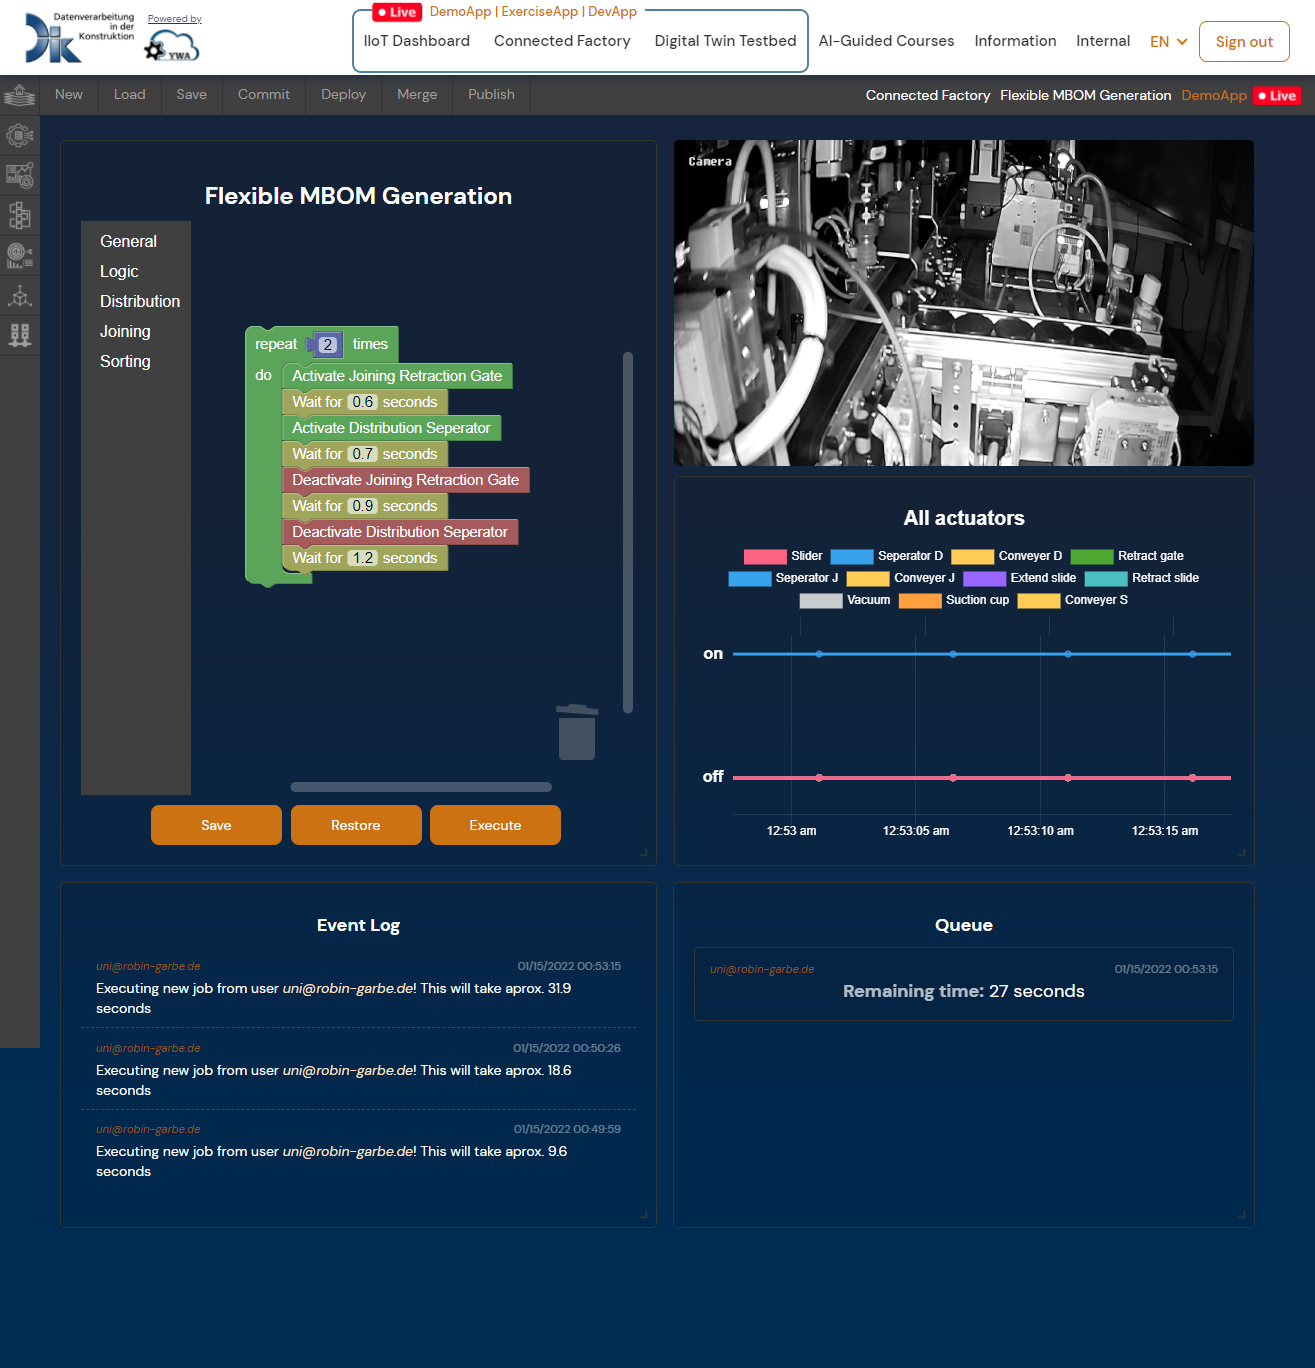
\includegraphics[width=1.0\textwidth]{images/anhang/Screenshot_Prozessplanung.png}
    \caption{Ganzseitiger Screenshot der Prozessplanungs und -steuerungs Seite}
    \label{fig:anhang_Screenshot_Prozessplanung}
\end{figure}
%
\begin{figure}[htbp]
	\centering\includegraphics[width=1.0\textwidth]{images/anhang/Screenshot_Übersichtsseite.png}
    \caption{Ganzseitiger Screenshot der Übersichts-Seite}
    \label{fig:anhang_Screenshot_Übersichtsseite}
\end{figure}
%
\begin{figure}[htbp]
	\centering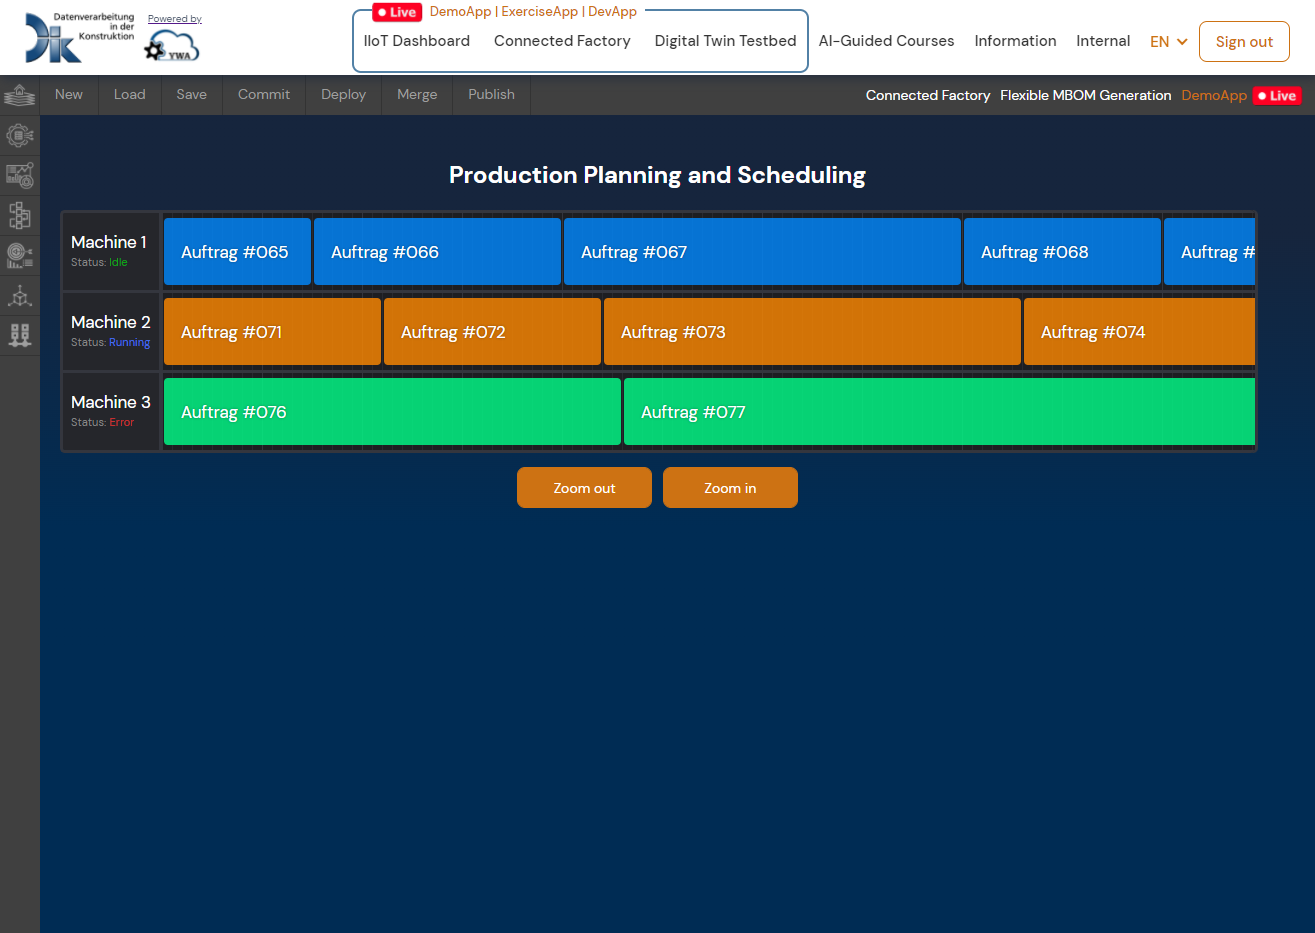
\includegraphics[width=1.0\textwidth]{images/anhang/Screenshot_Produktionsplanung.png}
    \caption{Ganzseitiger Screenshot der Produktionsplanungs-Seite}
    \label{fig:anhang_Screenshot_Produktionsplanung}
\end{figure}
